%harihiom
\documentclass{book}

\usepackage[english]{babel}
%\usepackage[utf8]{inputenc}
%\usepackage{amsmath}
\usepackage{graphicx}
\usepackage{comment}
\usepackage{float}
%\usepackage{wrapfig}
%\usepackage{titlepic}
%\usepackage[colorinlistoftodos]{todonotes}
\usepackage{graphicx,epstopdf}
\usepackage{amsmath,amssymb,amsfonts,subfigure}
\usepackage{comment}
\usepackage{algorithm}
\usepackage{algpseudocode}
\usepackage{pifont}
\usepackage[normalem]{ulem}
\usepackage[english]{babel}
\usepackage[utf8x]{inputenc}
\usepackage{graphicx}
\usepackage{calc}
\usepackage{graphicx}
\usepackage{subfigure}
\usepackage{gensymb}
\usepackage{url}
\usepackage[utf8x]{inputenc}
\usepackage{amsmath}
\usepackage{graphicx}
\graphicspath{{images/}}
\usepackage{parskip}
\usepackage{fancyhdr}
\usepackage{vmargin}
\usepackage{algorithm}
\linespread{1}
\usepackage{color}
\usepackage{cite}
\usepackage{amsmath,amssymb}
\newtheorem{claim1}{Claim}
\usepackage{algpseudocode}% http://ctan.org/pkg/algorithmicx
\usepackage[compatibility=false]{caption}% http://ctan.org/pkg/caption
\setmarginsrb{3 cm}{2.5 cm}{3 cm}{2.5 cm}{1 cm}{1.5 cm}{1 cm}{1.5 cm}

%\newtheorem{theorem}{Theorem}
%\newtheorem{lemma}{Lemma}

\title{Probability Ideas in Computing}

\begin{document}
\maketitle
\chapter{The Monty Hall Show}
The Monty Hall problem is an interesting basic probability brainteaser, named after the host (Monty Hall) of an American television reality show `Let's Make a Deal'. The problem was introduced by the American Statistician Steve Selvin, in his letter to the peer reviewed journal `American Statistician' \cite{selvin1975problem}. Before visiting the problem, let us understand a simpler basic probability scenario.  \\

\section{A Simple Scenario}
Assume you are the contestant of a reality show, presented with $3$ doors in front of you. Behind every door is exactly one out of the three items, $2$ goats and a BMW car. Being a contestant, you do not know the item each door hides. You are asked to choose any one of these $3$ doors and are gifted with the item the chosen door hides. Visibly, you are considered a winner if you choose the door hiding the BMW. Our basic knowledge of probability quickly tells us that \textit{the probability of winning = $1/3$ and probability of losing = $2/3$.}\\

\section{The Monty Hall Scenario}
Our smart statistician Steve now enters the scene, bringing a new twist to the scenario. First, he asks us to choose one door, absolutely similar to the simpler scenario discussed above. Again, similar to the simpler scenario, we choose one of the gates randomly. Now, out of the remaining two doors (not chosen by us), Steve opens the one hiding a goat\footnote{Steve knows which door hides what. That's why he is capable of opening a door which has a goat hidden.}. Since, there are two doors hiding goats; definitely, there is at least one goat hidden in the non chosen doors. Next, we are offered a chance to swap our choice and choose the third door which is unopened (previously not chosen by us). 
The question of interest is : \textbf{Should we swap our choice?} Do you think swapping makes any difference to our probability of winning? Refer Figure \ref{monty}. \\

\begin{figure}[h!]
\centering
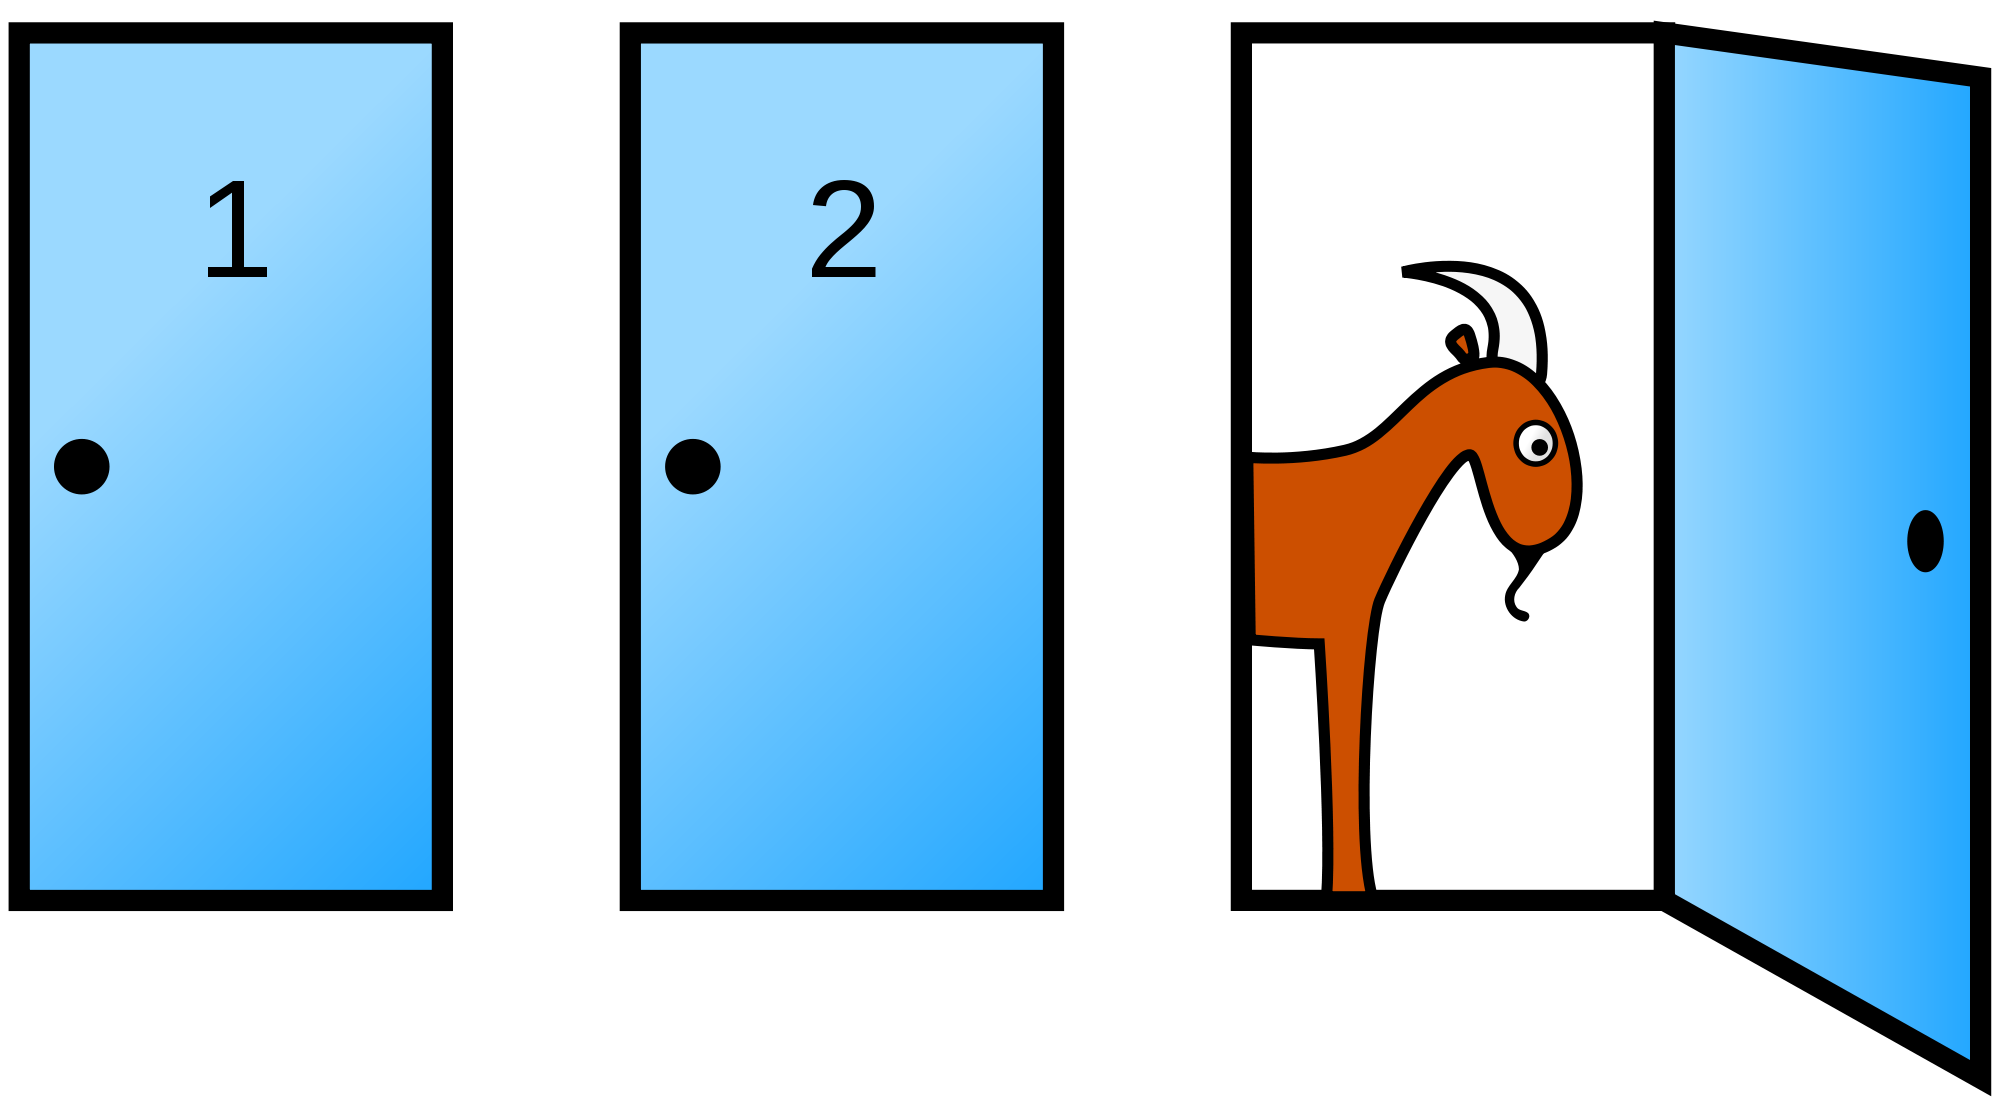
\includegraphics[width=0.5\textwidth]{monty.png}
\caption{\textbf{The Monty Hall Game}: Assume we have previously chosen door $1$. Now, Steve shows us a goat hidden in gate $3$. Next, we are presented with a posssibility of switching to door $2$.}
\label{monty}
\end{figure}

It appears that switching should not make any difference to our probability of winning. But to our surprise, the answer to this seemingly simple puzzle is : {\large{\textbf{We should always swap.}}} Swapping increases our chances of winning. 

\section{Swapping Increases the Chances of Winning}

Before discussing the reasoning behind the stated solution in detail, let us discuss a small intuition for this seemingly non trivial solution. 

\subsection{Proof idea}
It might appear to a reader that since one door hiding a goat has been opened by Steve, there are $2$ doors left - one with a BMW and another with a goat. The probability of BMW being in any of these doors is $1/2$. Hence, swapping or not swapping should not make any difference to our probability of winning. 

Now, carefully observe that when we initially choose a door (without having any additional knowledge), our probability of choosing a door with a goat was $2/3$. Hence, there is a greater chance that the door we are currently standing with holds a goat. Steve has now shown us another door hiding a goat. Hence, it is advisable to swap our choice since that increases our probability of choosing the door hiding a BMW. 

\subsection{Proof} 

Let us consider two cases; first where we swap the chosen door and another, where we don't. 

\subsubsection{Case 1 : We do not swap}
We choose one door randomly. Hence, the probability of choosing a goat is $2/3$ and that of choosing a BMW is  $1/3$. Next, Steve opens one of the doors hiding a goat. But, we have decided not to swap. Hence, the extra knowledge Steve just now revealed does not matter to us. Hence, our probability of winning is $1/3$ and that of losing is $2/3$.

\subsubsection{Case 2 : We swap}
We choose one door randomly. Hence, the probability of choosing a goat is $2/3$ and that of choosing a BMW is  $1/3$. Next, Steve opens one of the doors hiding a goat. we have decided to swap. Please note that if we have initially chosen a BMW, we will end up choosing a goat and vice versa. Hence, our probability of winning now depends on what we have chosen previously. There are two possible cases here, discussed below. 

\textbf{\textit{Case 2(a) :}} We have initially chosen a door containing a goat.\\ 
Probability (we have chosen a door containing a goat) = $2/3$. Now Steve shows us the other door having a goat. So, when we swap, we definitely pick the door hiding the BMW. Hence, our probability of winning = $2/3$. \\

\textbf{\textit{Case 2(b) : }}We have initially chosen the door containing BMW.\\ 
Probability (we have chosen the door containing BMW) = $1/3$. Now Steve shows us the other door having a goat. So, when we swap, we definitely pick the door having another goat. Hence, our probability of losing= $1/3$.\\

Hence, swapping the choice swaps our probabilities of winning and losing the game discussed in the basic scenario. So, we must always consider swapping.

\section{Generalisation of the puzzle}

Next, we generalise the puzzle. A player might consider swapping her choice with certain probability. Assume that a player decides to switch her choice with a probability $p$. What are the chances of winning and losing the game in this genaralised scenario?

Consider Figure \ref{modi}
\begin{figure}[h!]
\centering
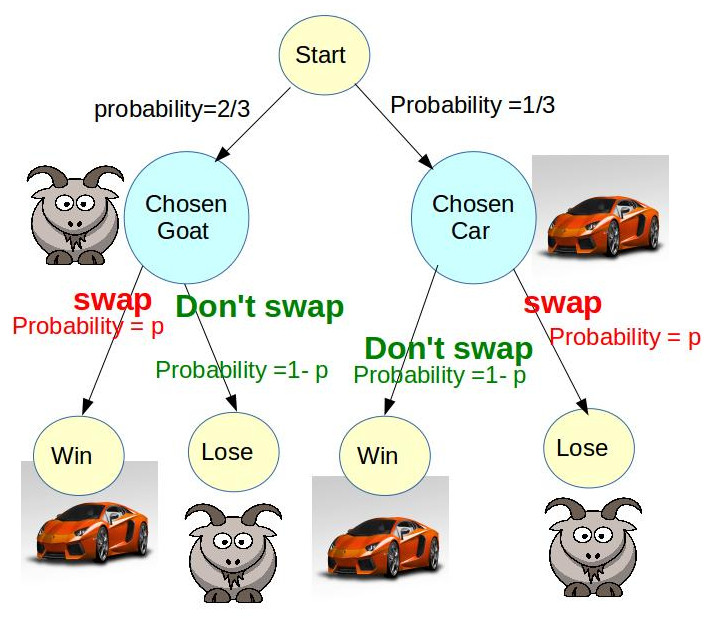
\includegraphics[width=0.7\textwidth]{goat.jpg}
\caption{Generalisation of Monty Hall Problem}
\label{modi}
\end{figure}

A keen reader would have observed by now that there are $2$ ways of winning the game.
\begin{itemize}
\item We initially choose the gate hiding a goat and later swap our choice. 
\item We initially choose the door hiding the BMW and later do not swap.
\end{itemize}

Hence, by the basic principles of probability, $Pr(Winning)$= $\frac{2}{3} \times p\ +\ \frac{1}{3} \times (1-p)$
= $\frac{1}{3}p + \frac{1}{3}$
= $\frac{1+p}{3}$

In a similar way, there are two ways in which we can lose the game.
\begin{itemize}
\item We initially choose the gate hiding a BMW and later swap our choice. 
\item We initially choose the door hiding the goat and later do not swap.
\end{itemize}

Again, by the basic principles of probability, $Pr(Losing)$= $\frac{1}{3} \times p\ +\ \frac{2}{3} \times (1-p)$
= $\frac{2}{3} - \frac{1}{3}p$
= $\frac{2-p}{3}$

The probability of losing the game can also be simply calculated as $Pr(Losing)\ =\ 1-Pr(Winning)$.

\textbf{We can easily note that the probability of winning can be maximised by choosing $p=1$, i.e., always swapping our choice.}


\section{Introduction to Random Variables}

The usage of random variables is at the heart of probaility and statistics. Random variables are very tightly coupled with random experiments and allow an easy quantification of their outcomes. 

\subsection{Definition}
A random variable can be defined as a function which maps the outcomes of a random experiment to numbers (typically real numbers). They can be defined as per our convinience. For example, consider the random experiment of tossing a coin. So, there are two possible outcomes of this experiment, getting a head and getting a tail. Now, a random variable can be used to associate a number with each of these outcomes as shown below. 
\[
X = \left\{\def\arraystretch{1.2}%
\begin{array}{@{}c@{\quad}l@{}}
19 & \text{if the coin shows up head}\\
10 & \text{if the coin shows up tail}\\
\end{array}\right.
\]\\

As a matter of fact, we could have used any two numbers instead of $19$ and $10$. Other interesting ways of defining random variables are:
 
\subsubsection{Tossing a coin multiple times and counting the occurences of head}
Toss a coin $100$ times and define the random variable $Y$ to be the number of times the coin shows up head. A keen reader would have observed that the range from which $Y$ can take values is $\{0,1,2,...,99,100\}$. 

\subsubsection{Rolling a die $10$ times and adding up the appeared numbers}
Roll a die $10$ times and define the random variable $Z$ to be the sum of the numbers which have appeared. Here, the range from which $Z$ takes values is $\{10,11,..............,60\}$. 

\subsection{Expected Value of a Random Variable}
The expected value of a random variable indicates its average value. For example, consider the random variable $X$ defined as follows. \\
Assume we toss a coin once. Head results in a payoff of $100$ points while tail offers no points. In this case, \\
\[
X = \left\{\def\arraystretch{1.2}%
\begin{array}{@{}c@{\quad}l@{}}
100 & \text{if the coin shows up head}\\
0 & \text{if the coin shows up tail}\\
\end{array}\right.
\]\\

We know by intuition that if we repeat this experiment again and again; once in two tosses, we will get a head (hence $100$ points). So, the expected value of $X$ is $50$ \footnote{Practically speaking, winning $50$ points is not possible because one can either win $100$ points or no point. But please note that we are talking about the expected value (on an average how much do you win?). This has been elaborated further in the case of Monty Hall problem in the upcoming section. }. Next, we define this notation of expected value rigorously. 

\textbf{Consider a random variable {\textcolor{blue}{$X$}} which can take the values {\textcolor{blue}{$x_1, x_2, ...., x_n$}} with probabilities {\textcolor{blue}{$p_1,p_2,...,p_n$}} respectively. Then the expected value of {\textcolor{blue}{$X$, $E[X]=x_1 \times p_1 + x_2 \times p_2 + ... + x_n \times p_n = \sum_{i=1}^{n} x_i p_i$}}.}\\

For the example discussed above, the expected number of points one wins, can simply be calculated as, $E[X] = 100 \times 0.5 + 0 \times 0.5$ = $50$ points. However, the expressions for calculating the expected values of random variables $Y$ and $Z$ gets dirtier. We will visit those expressions in the next chapter.   


\section{Random Variables and Monty Hall Problem}
Being acquainted with the definition of random variables, we can now define a random variable $X$ for the Monty Hall Problem. Let $X$ be defined as follows.\\
\[
X = \left\{\def\arraystretch{1.2}%
\begin{array}{@{}c@{\quad}l@{}}
100 & \text{if we choose the door hiding a car}\\
0 & \text{if we choose a door hiding a goat}\\
\end{array}\right.
\]\\

This means that we get $100$ points on winning a car and winning a goat offers nothing. Recall the basic scenario we discussed before Monty Hall problem (without the opportunity of switching). In that case, the expected amount of money one wins is, $E[X] = 100(1/3) + 0 (2/3) = 100/3$, which can also be interpreted in the following two ways. 

\begin{itemize}
\item If we play the game once, there is a $33.3\%$ chance that we will win. 
\item If we play the game again and again, we will win once in three times. 
\end{itemize}

Now consider the Monty Hall scenario where we are allowed switching our door after Steve shows us one hidden goat. We have seen that the probabilities of winning and losing gets swapped when one switches her choice. In that case, $E[X'] = 100(2/3) + 0 (1/3) = 200/3$, which means that there is a $66.6\%$ chance of winning. 

One can also extend this terminology for the generalised case of Monty Hall problem where switching was done with probability $p$ and obtain the result $E[X'']=100(1+p)/3$.


\bibliographystyle{plain}
\bibliography{book}

\end{document}
